% (find-LATEX "2021-2-C2-MT1.tex")
% (defun c () (interactive) (find-LATEXsh "lualatex -record 2021-2-C2-MT1.tex" :end))
% (defun C () (interactive) (find-LATEXsh "lualatex 2021-2-C2-MT1.tex" "Success!!!"))
% (defun D () (interactive) (find-pdf-page      "~/LATEX/2021-2-C2-MT1.pdf"))
% (defun d () (interactive) (find-pdftools-page "~/LATEX/2021-2-C2-MT1.pdf"))
% (defun e () (interactive) (find-LATEX "2021-2-C2-MT1.tex"))
% (defun o () (interactive) (find-LATEX "2021-2-C2-MT1.tex"))
% (defun u () (interactive) (find-latex-upload-links "2021-2-C2-MT1"))
% (defun v () (interactive) (find-2a '(e) '(d)))
% (defun d0 () (interactive) (find-ebuffer "2021-2-C2-MT1.pdf"))
% (defun cv () (interactive) (C) (ee-kill-this-buffer) (v) (g))
%          (code-eec-LATEX "2021-2-C2-MT1")
% (find-pdf-page   "~/LATEX/2021-2-C2-MT1.pdf")
% (find-sh0 "cp -v  ~/LATEX/2021-2-C2-MT1.pdf /tmp/")
% (find-sh0 "cp -v  ~/LATEX/2021-2-C2-MT1.pdf /tmp/pen/")
%     (find-xournalpp "/tmp/2021-2-C2-MT1.pdf")
%   file:///home/edrx/LATEX/2021-2-C2-MT1.pdf
%               file:///tmp/2021-2-C2-MT1.pdf
%           file:///tmp/pen/2021-2-C2-MT1.pdf
% http://angg.twu.net/LATEX/2021-2-C2-MT1.pdf
% (find-LATEX "2019.mk")
% (find-CN-aula-links "2021-2-C2-MT1" "2" "c2m212mt1" "c2mt1")
%
% Video (not yet):
% (find-ssr-links      "c2m212mt1" "2021-2-C2-MT1")
% (code-eevvideo       "c2m212mt1" "2021-2-C2-MT1")
% (code-eevvideo-local "c2m212mt1" "2021-2-C2-MT1")
% (find-c2m212mt1video "0:00")

% «.defs»		(to "defs")
% «.title»		(to "title")
% «.regras»		(to "regras")
% «.itens-a-b-c»	(to "itens-a-b-c")
% «.gabarito»		(to "gabarito")
%
% «.djvuize»		(to "djvuize")

\documentclass[oneside,12pt]{article}
\usepackage[colorlinks,citecolor=DarkRed,urlcolor=DarkRed]{hyperref} % (find-es "tex" "hyperref")
\usepackage{amsmath}
\usepackage{amsfonts}
\usepackage{amssymb}
\usepackage{pict2e}
\usepackage[x11names,svgnames]{xcolor} % (find-es "tex" "xcolor")
\usepackage{colorweb}                  % (find-es "tex" "colorweb")
%\usepackage{tikz}
%
% (find-dn6 "preamble6.lua" "preamble0")
%\usepackage{proof}   % For derivation trees ("%:" lines)
%\input diagxy        % For 2D diagrams ("%D" lines)
%\xyoption{curve}     % For the ".curve=" feature in 2D diagrams
%
\usepackage{edrx21}               % (find-LATEX "edrx21.sty")
\input edrxaccents.tex            % (find-LATEX "edrxaccents.tex")
\input edrx21chars.tex            % (find-LATEX "edrx21chars.tex")
\input edrxheadfoot.tex           % (find-LATEX "edrxheadfoot.tex")
\input edrxgac2.tex               % (find-LATEX "edrxgac2.tex")
%
%\usepackage[backend=biber,
%   style=alphabetic]{biblatex}            % (find-es "tex" "biber")
%\addbibresource{catsem-slides.bib}        % (find-LATEX "catsem-slides.bib")
%
% (find-es "tex" "geometry")
\usepackage[a6paper, landscape,
            top=1.5cm, bottom=.25cm, left=1cm, right=1cm, includefoot
           ]{geometry}
%
\begin{document}

%\catcode`\^^J=10
%\directlua{dofile "dednat6load.lua"}  % (find-LATEX "dednat6load.lua")

% %L dofile "edrxtikz.lua"  -- (find-LATEX "edrxtikz.lua")
% %L dofile "edrxpict.lua"  -- (find-LATEX "edrxpict.lua")
% \pu

% «defs»  (to ".defs")
% (find-LATEX "edrx21defs.tex" "colors")
% (find-LATEX "edrx21.sty")

\def\drafturl{http://angg.twu.net/LATEX/2021-2-C2.pdf}
\def\drafturl{http://angg.twu.net/2021.2-C2.html}
\def\draftfooter{\tiny \href{\drafturl}{\jobname{}} \ColorBrown{\shorttoday{} \hours}}



%  _____ _ _   _                               
% |_   _(_) |_| | ___   _ __   __ _  __ _  ___ 
%   | | | | __| |/ _ \ | '_ \ / _` |/ _` |/ _ \
%   | | | | |_| |  __/ | |_) | (_| | (_| |  __/
%   |_| |_|\__|_|\___| | .__/ \__,_|\__, |\___|
%                      |_|          |___/      
%
% «title»  (to ".title")
% (c2m212mt1p 1 "title")
% (c2m212mt1a   "title")

\thispagestyle{empty}

\begin{center}

\vspace*{1.2cm}

{\bf \Large Cálculo 2 - 2021.2}

\bsk

Mini-teste 1

\bsk

Eduardo Ochs - RCN/PURO/UFF

\url{http://angg.twu.net/2021.2-C2.html}

\end{center}

\newpage

% «regras»  (to ".regras")
% (c2m212mt1p 2 "regras")
% (c2m212mt1a   "regras")

As regras vão ser as mesmas dos

mini-testes dos semestres anteriores:

\ssk

{\footnotesize

% (c2m202mt1p 2 "regras")
% (c2m202mt1a   "regras")
\url{http://angg.twu.net/LATEX/2020-2-C2-MT1.pdf#page=2}

}

(Leia com muita atenção!!!!!!!!!!!)

\bsk

As questões vão ser disponibilizadas às 20:45 da sexta

12/novembro/2021 e vocês vão ter até as 20:45 do sábado

13/novembro/2021 pra entregar as respostas.

\newpage

Vamos usar a mesma função $f(x)$ do exercício 12...

Esta aqui:

% (c2m212somas1p 21 "exercicio-12")
% (c2m212somas1a    "exercicio-12")
% (find-latexscan-links "C2" "20211111_somas_1_ex_12")
% (find-xpdf-page "~/LATEX/2021-2-C2/20211111_somas_1_ex_12.pdf")
\centerline{$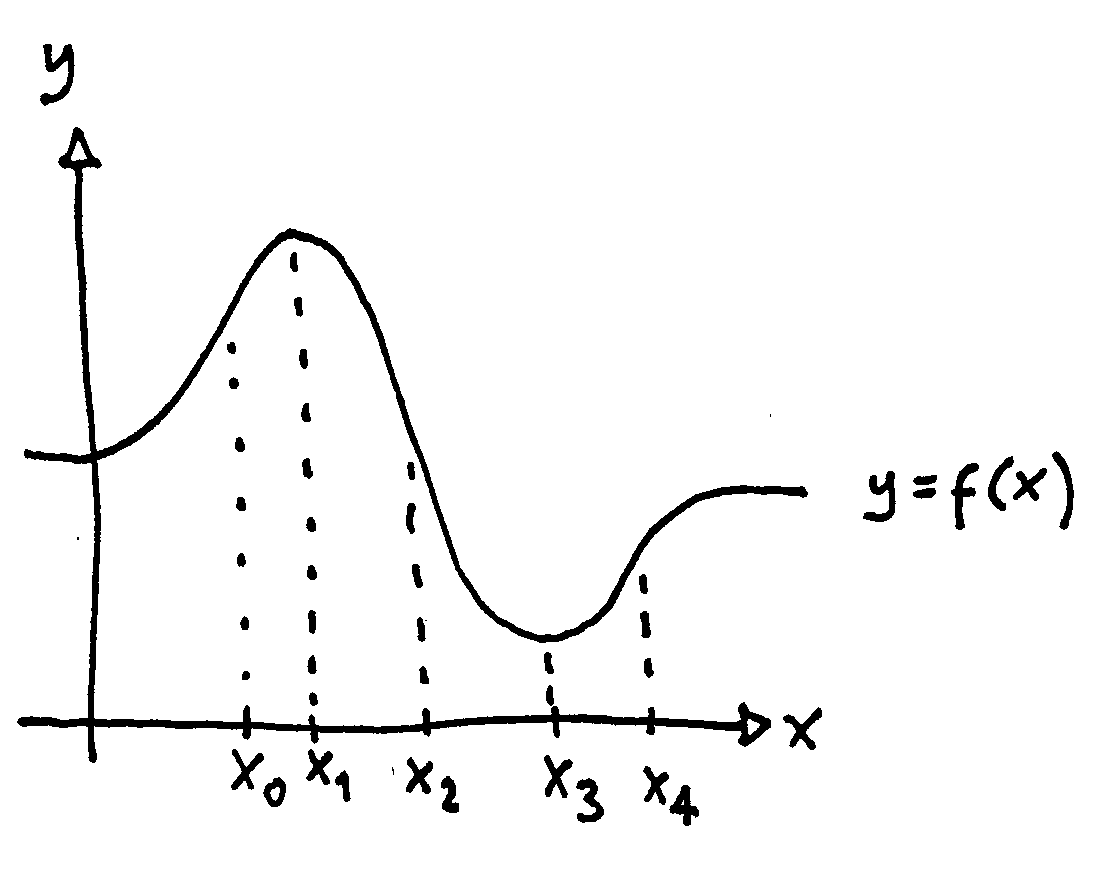
\includegraphics[height=5cm]{2021-2-C2/20211111_somas_1_ex_12.pdf}$}


Faça uma cópia dela à mão para cada item do mini-teste.

Não tem problema se as cópias ficarem meio tortas.

\newpage

% «itens-a-b-c»  (to ".itens-a-b-c")
% (c2m212mt1p 4 "itens-a-b-c")
% (c2m212mt1a   "itens-a-b-c")

\def\r#1{(\frac{#1}{2})}
\def\F#1{f(x_#1)}
\def\G#1#2{\r{f(x_#1)+f(x_#2)}}
\def\H#1#2{f(x_#2)-f(x_#1)}
\def\H#1#2{  x_#2 -  x_#1 }
\def\T#1#2{\G#1#2(\H#1#2)}

a) (0.1 pts) Represente graficamente sobre a primeira cópia:

\ssk

$  \F1(x_1-x_0)
 + \F2(x_2-x_1)
 + \F3(x_4-x_2)
$

\bsk

b) (0.1 pts) Represente graficamente sobre a segunda cópia:

\ssk

$  \F0(x_1-x_0)
 + \F1(x_2-x_1)
 + \F4(x_4-x_2)
$

\bsk

c) (0.3 pts) Represente graficamente sobre a terceira cópia

a interpretação da expressão abaixo como trapézios

\ColorRed{e} a interpretação dela como retângulos:

\msk

$\begin{array}{c}\T01 \\ + \; \T12 \\ \; + \T24\end{array}$


\newpage

% «gabarito»  (to ".gabarito")
% (c2m212mt1p 5 "gabarito")
% (c2m212mt1a   "gabarito")

{\bf Gabarito:}


\def\incgr#1{$\myvcenter{\includegraphics[height=2cm]{#1}}$}
\def\incgr#1{\;\;\; $\myvcenter{\includegraphics[height=2cm]{#1}}$}
\def\incgr#1{\;\;\; $\myvcenter{\includegraphics[height=3.5cm]{#1}}$}
\def\incgr#1{$\myvcenter{\includegraphics[height=3.5cm]{#1}}$}

\begin{tabular}{lll}
  %
  a)
  % (find-latexscan-links "C2" "20211111_somas_1_ex_12_mt1_a")
  % (find-xpdf-page "~/LATEX/2021-2-C2/20211111_somas_1_ex_12_mt1_a.pdf")
  \incgr{2021-2-C2/20211111_somas_1_ex_12_mt1_a.pdf}
  &
  b)
  % (find-latexscan-links "C2" "20211111_somas_1_ex_12_mt1_b")
  % (find-xpdf-page "~/LATEX/2021-2-C2/20211111_somas_1_ex_12_mt1_b.pdf")
  \incgr{2021-2-C2/20211111_somas_1_ex_12_mt1_b.pdf}
  \\
  c)
  % (find-latexscan-links "C2" "20211111_somas_1_ex_12_mt1_c")
  % (find-xpdf-page "~/LATEX/2021-2-C2/20211111_somas_1_ex_12_mt1_c.pdf")
  \incgr{2021-2-C2/20211111_somas_1_ex_12_mt1_c.pdf}
\end{tabular}


\newpage

Obs: tinha um error de digitação na questão (a)...

Compare:

$  \F1(x_1-x_0)
 + \F2(x_2-x_1)
 + \F3(x_4-x_2)
$

$  \F1(x_1-x_0)
 + \F2(x_2-x_1)
 + \F4(x_4-x_2)
$

Eu queria ter escrito a segunda, com $f(x_4)$,

mas me distraí e escrevi a primeira, com $f(x_3)$.

\ssk

O gabarito da (a) no slide anterior corresponde

à expressão com $f(x_4)$.


\GenericWarning{Success:}{Success!!!}  % Used by `M-x cv'

\end{document}

%  ____  _             _         
% |  _ \(_)_   ___   _(_)_______ 
% | | | | \ \ / / | | | |_  / _ \
% | |_| | |\ V /| |_| | |/ /  __/
% |____// | \_/  \__,_|_/___\___|
%     |__/                       
%
% «djvuize»  (to ".djvuize")
% (find-LATEXgrep "grep --color -nH --null -e djvuize 2020-1*.tex")

 (eepitch-shell)
 (eepitch-kill)
 (eepitch-shell)
# (find-fline "~/2021.2-C2/")
# (find-fline "~/LATEX/2021-2-C2/")
# (find-fline "~/bin/djvuize")

cd /tmp/
for i in *.jpg; do echo f $(basename $i .jpg); done

f () { rm -v $1.pdf;  textcleaner -f 50 -o  5 $1.jpg $1.png; djvuize $1.pdf; xpdf $1.pdf }
f () { rm -v $1.pdf;  textcleaner -f 50 -o 10 $1.jpg $1.png; djvuize $1.pdf; xpdf $1.pdf }
f () { rm -v $1.pdf;  textcleaner -f 50 -o 20 $1.jpg $1.png; djvuize $1.pdf; xpdf $1.pdf }

f () { rm -fv $1.png $1.pdf; djvuize $1.pdf }
f () { rm -fv $1.png $1.pdf; djvuize WHITEBOARDOPTS="-m 1.0 -f 15" $1.pdf; xpdf $1.pdf }
f () { rm -fv $1.png $1.pdf; djvuize WHITEBOARDOPTS="-m 1.0 -f 30" $1.pdf; xpdf $1.pdf }
f () { rm -fv $1.png $1.pdf; djvuize WHITEBOARDOPTS="-m 1.0 -f 45" $1.pdf; xpdf $1.pdf }
f () { rm -fv $1.png $1.pdf; djvuize WHITEBOARDOPTS="-m 0.5" $1.pdf; xpdf $1.pdf }
f () { rm -fv $1.png $1.pdf; djvuize WHITEBOARDOPTS="-m 0.25" $1.pdf; xpdf $1.pdf }
f () { cp -fv $1.png $1.pdf       ~/2021.2-C2/
       cp -fv        $1.pdf ~/LATEX/2021-2-C2/
       cat <<%%%
% (find-latexscan-links "C2" "$1")
%%%
}

f 20201213_area_em_funcao_de_theta
f 20201213_area_em_funcao_de_x
f 20201213_area_fatias_pizza



%  __  __       _        
% |  \/  | __ _| | _____ 
% | |\/| |/ _` | |/ / _ \
% | |  | | (_| |   <  __/
% |_|  |_|\__,_|_|\_\___|
%                        
% <make>

 (eepitch-shell)
 (eepitch-kill)
 (eepitch-shell)
# (find-LATEXfile "2019planar-has-1.mk")
make -f 2019.mk STEM=2021-2-C2-MT1 veryclean
make -f 2019.mk STEM=2021-2-C2-MT1 pdf

% Local Variables:
% coding: utf-8-unix
% ee-tla: "c2mt1"
% ee-tla: "c2m212mt1"
% End:
